\documentclass[10pt,b5paper,twoside,openany]{book}
% openany - normally chapters start at right page. That leads to blank pages if the content does not allow the chapter
% to start at the right page. openany function allows chapters to start at any page
%======================================================================
%>>>>>>> PACKAGES
\usepackage[utf8]{inputenc} %utf8 option to match Editor encoding
\usepackage[T1]{fontenc}  %some font encoding package
\usepackage{lmodern} %package that defines the font itself, allows polish letters
\usepackage{graphicx} %allows adding graphics to the document
\usepackage{wrapfig} %allows to create objects surrounded by text
\usepackage{amsmath,amsfonts,amssymb} %more math symbols, like matrices etc.
\usepackage[rightcaption]{sidecap} %allows to add captions at right and left sides of the figure, needs to be packed
%into the figure environment
\usepackage{float} %allows to specify floating options in some environments
\usepackage[margin=0.5in]{geometry} %margins
\usepackage{hyperref} %hyperlinks
\usepackage{xcolor} %
\usepackage{fancyvrb} %adds new types of verbatims
\usepackage{tcolorbox}
\usepackage{titlesec} %allows titling customization

\usepackage[acronym,toc,section=section]{glossaries}

%
% acronym - allows create different table for acronyms
% toc,section=section - allows glossaries to be printed in table of contents

\tcbuselibrary{skins,breakable} %probably for propper working of these black environments that code from VS is written in
%==========================================================================
% >>>>>>> DEFs
\def\bs{\textbackslash}
\def\us{\textunderscore}
\def\source_space{\vspace{0.2em}}

% >>>>>>> DEFINECOLORS
% href colors
\definecolor{hrefurl}{RGB}{46,71,217}
\definecolor{hreflink}{RGB}{39,117,15}

% >>>>>>> NEWENVIRONMENTS
% this is a custom verbatim with black background
\newenvironment{BGVerbatim}
 {\VerbatimEnvironment
  \begin{tcolorbox}[
    breakable,
    colback=vsblack,
    spartan
    ]%
  \begin{Verbatim}}
 {\end{Verbatim}\end{tcolorbox}}
 
% >>>>>>> NEWCOMMANDS
\newcommand{\tc}[2]{\textcolor{#1}{#2}}
\newcommand{\ul}[1]{\underline{#1}}
\newcommand{\myline}[2]{\noindent\makebox[\linewidth]{\rule{#1cm}{#2pt}}}
\newcommand{\keyshortcut}[1]{\texttt{#1}}
%==========================================================================
% >>>>>>> SETTINGS
\hypersetup %edytuje właściwości hiperłączy np. kolor
{
colorlinks=true,
linkcolor=black,
urlcolor=hrefurl
}

% \pagestyle{empty} %sprawia ze strony nie są numerowane - jezeli jest na stronie \maketitle to style jest nadpisywany i na takiej stronie trzeba dodatkowo umiescic zaraz po \maketitle komende \thispagestyle{empty}

\parindent 0px %ustawia wartość wcięcia na początku akapitu/paragrafu na zero, co daje taki efekt, że nie ma wcięć

\titleformat{\part}{\bfseries\centering\Huge{\titlerule[1.5pt]\vspace{0.1em}\titlerule[1.5pt]\vspace{0.5em}}}{Part \thepart\ -}{10pt}{\Huge}[{\vspace{0.5em}\titlerule[1.5pt]\vspace{0.1em}\titlerule[1.5pt]}]
\titlespacing{\part}{0pt}{0pt}{20pt}

\titleformat{\chapter}{\bfseries\centering\Huge{\titlerule[1.5pt]}}{\thechapter .}{10pt}{\huge}[{\titlerule[1.5pt]}]
\titlespacing{\chapter}{0pt}{0pt}{20pt}

\titleformat{\section}{\bfseries\large}{\thesection}{0.5em}{}[\titlerule]
\titlespacing{\section}{0pt}{1ex}{10pt} %how to use "plus" operator

\makeglossaries %>>>>>>>>>>>>>>>>>>>>>>>>>>>>>>>>>>>GLOSSARIES

%glossary entries examples:

%\newglossaryentry{paradigm}
%{
   % name=paradigm,
    %description={a typical example or pattern of something; a pattern or model}
%}

%\newacronym{cpu}{CPU}{Central Processing Unit}


\newglossaryentry{miktex}
{
name=MiKTeX ,
description={a free and open-source distribution of the TeX/\LaTeX typesetting system for Microsoft Windows}
}

\newglossaryentry{bibtex}
{
name=BibTeX ,
description={a reference management software for formatting lists of references. The BibTeX tool is typically used together with the \LaTeX document preparation system}
}

\newglossaryentry{gls-ctan} %% glossary connected with below acronym
{
name=Comprehensive TeX Archive Network,
description={the authoritative place where TeX related material and software can be found for download}
}
\newacronym[see={[Glossary:]{gls-ctan}}]{ctan}{CTAN}{Comprehensive TeX Archive Network\glsadd{gls-ctan}}

%>>>>>>>>>>>>>>>>>>>>>>>>>>>>>>>>>>>>>>>>>>>>>>>GLOSSARIES-END

\date{\vspace{-3em}}
\title{\vspace{-2em}{\Huge \texttt{>> Computer Science <<}}\vspace{-0.5em}}
\author{{\LARGE Created and typeset by: Tomasz Zdeb}}
%adding some negative vspace allows to remove unnecessary blank space

\begin{document} %>>>>>>> PREAMBLE END
\maketitle
% \thispagestyle{empty} % \maketitle nadpisuje dzialanie \pagestyle{empty} dlatego musimy zaraz po tej komendzie skorzystać z ustawienia dla tej konkretnej strony

\tableofcontents
\newpage

\part{\LaTeX}

\chapter{General}

\section{Glossaries}

\Glspl{glossary} are being defined as ``\textit{an alphabetical list of words related to a specific subject, text, or dialect, with explanations; a brief dictionary}". To automate \glspl{glossary} generation and maintenence, \LaTeX\ uses a package called: \textbf{\glspl{glossary}}. Like in most cases, it is sometimes desired to specify additional \glspl{parameter} to the package, e.g. \textit{acronym}, \textit{toc}, \textit{section=section}. Which will be explained later in this section.\\

Before processing any code two things have to be mentioned. One: \glspl{glossary} package require \textbf{\href{https://www.perl.org/}{Perl}} interpreter to be present at the machine. Two: the package requires custom compilation scheme in order to take effect. Unfortunately there is no preset built into \textbf{\href{https://www.xm1math.net/texmaker/}{TeXMaker}} environment for a compilation scheme that will proces glossaries. A custom command \gls{pipeline} has to be configured manually.

\begin{figure}[H]
\centering
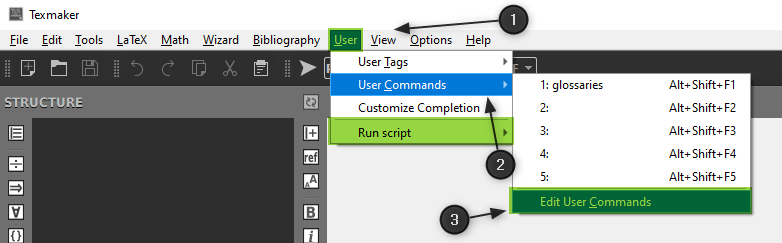
\includegraphics[scale=0.6]{content/LaTeX/figures/user_command_glossaries_marked.png}
\caption{Location of \textbf{Edit User Commands} button in \textbf{\href{https://www.xm1math.net/texmaker/}{TeXMaker}} environment}
\end{figure}

In order to define the custom command \gls{pipeline}, go to: \textbf{User} -> \textbf{User Commands} -> \textbf{Edit User Commands} and type below code into \textbf{command} field:
%\vspace{-0.5em} --------------------------------------------------------------------
\begin{verbatim}
pdflatex -synctex=1 -interaction=nonstopmode %.tex | makeglossaries % | pdflatex 
-synctex=1 -interaction=nonstopmode %.tex | "C:/Program Files (x86)/Adobe/Acrobat
Reader DC/Reader/AcroRd32.exe" %.pdf
\end{verbatim}

\begin{figure}[H]
\centering
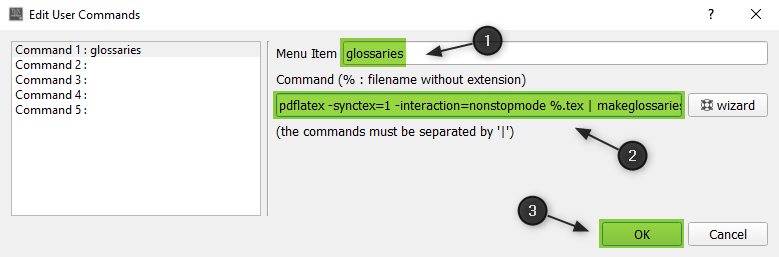
\includegraphics[scale=0.6]{content/LaTeX/figures/custom_command_marked.png}
\caption{Layout of \textbf{Edit User Commands} window in \textbf{\href{https://www.xm1math.net/texmaker/}{TeXMaker}} environment}
\end{figure}

Pipe symbol is used to chain commands. Words preceded by pause: ``-'' are \glspl{parameter} passed to commands, which are words without any additions, placed at the beginning of every part - right after pipe or at the very beginning. Disassembly of this chain of commands allows to differentiate four differents parts here:
\begin{enumerate}
\item Generate \textbf{.pdf} file from the \textbf{.tex} file
\item Generate \glspl{glossary}
\item Generate \textbf{.pdf} file from the \textbf{.tex} file
\item Display \textbf{.pdf}
\end{enumerate}

There are two types of entries that \gls{glossary} package provides by default:
\begin{itemize}
\item \glspl{glossary}
\item acronyms
\end{itemize}

\Glspl{glossary} are being defined in the preamble after \texttt{\bs makeglossaries} command that has to be put before any of the entries. Syntax of an \gls{glossary} and acronym entry is as shown below.

\begin{figure}[H]
\centering
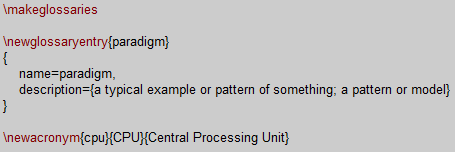
\includegraphics[scale=1.0]{content/LaTeX/figures/glossary_definition.png}
\caption{Commands used to define \glspl{glossary} and acronyms}
\label{fig:glossary_definition}
\end{figure}

To print a list of \glspl{glossary}, \texttt{\bs printglossary} command is used. For an entry to be printed on the list, at least one reference to it in the text is needed. Otherwise even if defined in the preamble, the entry won't be printet on the list.

\begin{figure}[H]
\centering
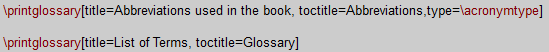
\includegraphics[scale=1.0]{content/LaTeX/figures/printglossary.png}
\caption{Commands used to print \gls{glossary} and acronym list}
\label{fig:printglossary}
\end{figure}

By default a list containing both \glspl{glossary} and acronyms is printed. As shown later on figure \ref{fig:usepackage_glossaries} \gls{parameter} \texttt{acronym} can be provided while invoking the package use, that allows to print separate list for acronyms and \glspl{glossary}. To print the separate list for acronyms specify \texttt{type=\bs acronymtype} attribute in a separate \texttt{\bs printglossary} call as shown on figure \ref{fig:printglossary}, which also illustrate, how a custom title\footnote{Title displayed in the text} as well as token title\footnote{Title displayed in table of content} can be set. To allow \gls{glossary} table to be included in table of contents an additional parameters: \texttt{toc} and \texttt{section=section} are needed when invoking \textbf{\glspl{glossary}} package as shown on picture \ref{fig:usepackage_glossaries}.

\begin{figure}[H]
\centering
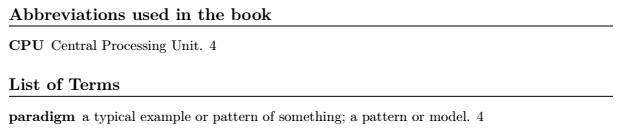
\includegraphics[scale=0.8]{content/LaTeX/figures/glossary_types.png}
\caption{Lists of acronyms and glossaries generated separately with use of \textbf{acronym} parameter for \textbf{\glspl{glossary}} package, that allows for separate list for acronyms to be printed}
\end{figure}

To reference a \gls{glossary} or acronym, several commands are used.

\begin{figure}[H]
\centering
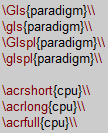
\includegraphics[scale=1.0]{content/LaTeX/figures/reference_glossaries.png}
\caption{Commands used to reference \glspl{glossary} and acronyms}
\end{figure}

Each entry can be referenced in several ways. Plural and singular forms as well as upper case and lowercase versions are avaliable for \glspl{glossary}. Acronym references differ from each other by level of detail printed.

\begin{figure}[H]
\centering
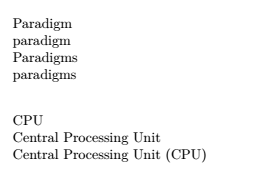
\includegraphics[scale=1.0]{content/LaTeX/figures/glossary_calls.png}
\caption{Examples of \glspl{glossary} and acronyms references}
\end{figure}

\begin{figure}[H]
\centering

\includegraphics[scale=1.0]{content/LaTeX/figures/usepackage_glossaries.png}
\caption{Command used to invoke the use of \textbf{glossaries} package with additional parameters passed to it}
\label{fig:usepackage_glossaries}
\end{figure}

There are many more options regarding to \gls{glossary} package, i.e. commands used to customize display of the \gls{glossary}, enable sorting, create custom \glspl{glossary}, put alternative text in references to a \gls{glossary}, define custom spelling for plural form, etc. You can find them on \acrshort{ctan} \href{https://www.ctan.org/pkg/glossaries}{website}~\cite{ctan_glossaries}.

\section{Bibliography}

In order to automate the process, make it more flexible and easily maintainable, there is a bibliography processor shipped with \Gls{miktex}, called \textbf{\Gls{bibtex}}. In general \textbf{\Gls{bibtex}} is considerd to be standalone tool, but in real life practice, it has very few uses, beside being bibliography management system for \LaTeX distributions. Thus it's very convinient to include it in \Gls{miktex} package by default.

\Gls{bibtex} itself alows to create citations to specified bibliography. It also contains built in bibliography listing functionality with predefined styles, that can be overriden.

\begin{figure}[H]
\centering
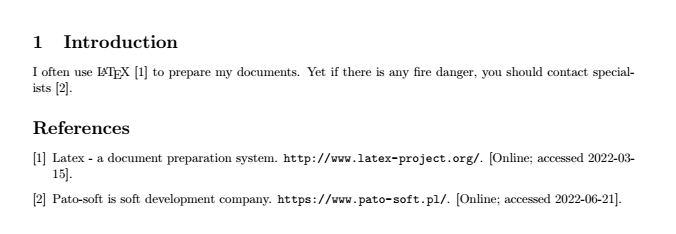
\includegraphics[scale=0.75]{content/LaTeX/figures/biblio_outcome.png}
\caption{An example showing default style of bibliography listing with citations generated by \gls{bibtex}}
\label{fig:bibliography_example}
\end{figure}

Bibliography items are stored in a dedicated files with \textbf{\gls{bib}} extension, that have to follow certain criteria. \textbf{\gls{bib}} files are organized in a key-value dictionary.

\begin{figure}[H]
\centering
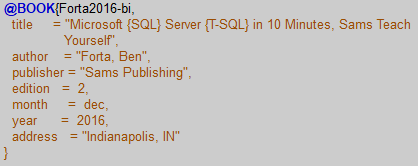
\includegraphics[scale=0.9]{content/LaTeX/figures/biblio_example.png}
\caption{Structure of a bibliography item entry in a \gls{bib} file}
\label{fig:biblio_example}
\end{figure}

\fbox{\textcolor{red}{FINISH THIS CHAPTER}}

\begin{figure}[H]
\centering
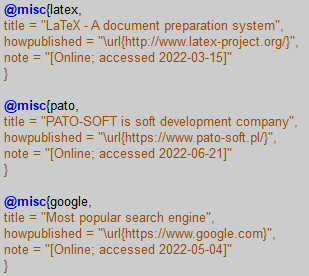
\includegraphics[scale=0.9]{content/LaTeX/figures/biblio_bib.png}
\caption{Add caption}
\label{fig:printglossary} % change label
\end{figure}

\begin{figure}[H]
\centering
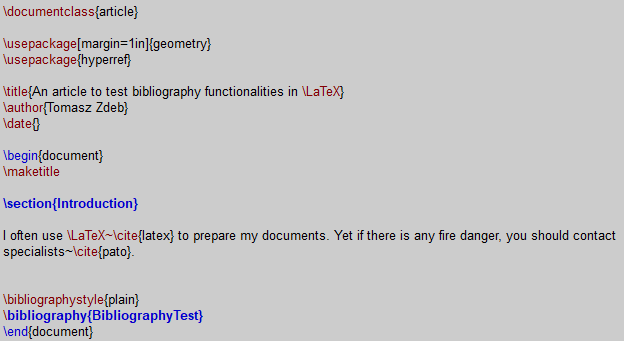
\includegraphics[scale=0.6]{content/LaTeX/figures/biblio_latex.png}
\caption{Add caption}
\label{fig:printglossary} % change label
\end{figure}

\begin{figure}[H]
\centering
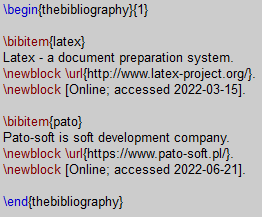
\includegraphics[scale=0.9]{content/LaTeX/figures/biblio_bbl.png}
\caption{Add caption}
\label{fig:printglossary} % change label
\end{figure}

Some quick guides, as well as some converters can be found \href{https://www.bibtex.com/g/bibtex-format/}{here}. Additional information can be found on the official \href{https://tug.org/bibtex/}{website}.\\

Advanced users may want to create a bibliography after each parto or chapter. Detailed guid on how to achieve such effets can be found \href{https://tex.stackexchange.com/questions/229846/different-bibliographies-for-each-chapter-with-shared-references}{here}

\section{Quotes}

There are several types of quoting avaliable in \LaTeX.

\textbf{French quotes}

\textbf{German quotes}

\textbf{Polish quotes}

\textbf{Anglo-Saxon quotes}

Symbol that is placed on the same key as \textbf{tilde} (under or next to the \textbf{escape} button), is used to generate right facing quotes used in anglo-saxon quoting notation.

\fbox{\textcolor{red}{FINISH THIS CHAPTER}}

\section{Listing environments}

\fbox{\textcolor{red}{FINISH THIS CHAPTER}}

Next to \textbf{Itemize} and \textbf{Enumerate} there is \textbf{Description} list environment in \LaTeX . It's a glossary type of list environment consisting of key-value data records. e.g.

\begin{description}
\item[Item one] description of item one
\item[item two] description of item two
\item[item three] description of item three
\end{description} 

Above structure is generated by code:

\begin{verbatim}
\begin{description}
\item[Item one] description of item one
\item[item two] description of item two
\item[item three] description of item three
\end{description} 
\end{verbatim}

\section{Where to inser captions and labels}
\fbox{\textcolor{red}{remember to surround tables, figures etc. in their wrapper floatin environments like figure, table etc. and add the caption and label}}
\section{How to avoid a line break}
\fbox{\textcolor{red}{to instruct \LaTeX no to break line between some content use tilde, e.g. no\textasciitilde line\textasciitilde break}}
\section{How to generate tilde}
\fbox{\textcolor{red}{FINISH THIS CHAPTER}}
\section{Differences between ref and hred referencing}
\fbox{\textcolor{red}{FINISH THIS CHAPTER}}
\section{MikTeX standard files}
\fbox{\textcolor{red}{FINISH THIS CHAPTER}}
\begin{verbatim}
C:\Program Files\MiKTeX\tex\latex\base
\end{verbatim}
\section{TO DOs}
\fbox{\textcolor{red}{Add list of tables and list of figures to the table}}\\
\fbox{\textcolor{red}{Add bibliography to the list of contents}}\\
\fbox{\textcolor{red}{Add non numbered chapter: acronyms and glossaries to table of contents}}\\
\fbox{\textcolor{red}{Go through the whole document and add lacking glossary/acronym entries}}\\
\fbox{\textcolor{red}{Go through the whole document and add lacking bibliography entries}}\\
\fbox{\url{http://www.peteryu.ca/tutorials/publishing/latex_captions}}\\
\fbox{\url{https://tex.stackexchange.com/questions/229846/different-bibliographies-for-each-chapter-with-shared-references}}\\
\fbox{\url{https://ctan.org/pkg/multirow}}\\
\fbox{\url{https://dictionary.cambridge.org/pl/dictionary/english/glossary}}\\
\fbox{\url{https://tex.stackexchange.com/questions/17653/how-to-list-all-bibliography-entries-without-citing}}\\
\fbox{\url{https://www.overleaf.com/learn/latex/Algorithms}}\\
\fbox{\url{https://tex.stackexchange.com/questions/1669/resuming-a-list}}\\

 %LaTeX Part

\part{Windows}

\subsubsection{Key Shortcuts}
\begin{itemize}
\item \keyshortcut{<Ctrl + R>} - starts \textbf{run window}
\item \keyshortcut{<Win + Shift + S>} runs \textbf{Snip \& Sketch} (screenshot)
\fbox{WIN + . - emoji menu}
\end{itemize}

\subsection{Run Commands}
\begin{itemize}
\item \keyshortcut{Run -> taskmgr} - runs \textbf{Task Manager}
\item \keyshortcut{Run -> winver} - runs simple program displaying \textbf{Windows} version on current machine
\item \keyshortcut{Run -> mspaint} - runs \textbf{Paint}
\item \keyshortcut{Run -> calc} - runs \textbf{Calculator}
\item \keyshortcut{Run -> control} - runs \textbf{Control Panel}
\end{itemize}

\subsection{Windows register}
\textcolor{red}{change the article - what registry is used for?}

It's a system database that contains most of systems configuration options. User or system settings as well as applications setting are stored in the register. Before \textbf{Windows 95} \texttt{.ini} configurations files were used (similarly to linux), but later all of the configuration data is stored in register. To modify the register a dedicated editor is used, passing \texttt{regedit} to \textbf{Windows Run} will launch it.\\

\fbox{ WARNING - Do not do things listed below! they're shown just for educational purposes}\\

\textbf{Adding control panel to context menu}
\begin{itemize}
\item find \texttt{HKEY{\us}CLASSES{\us}ROOT{\bs}Directory{\bs}Background{\bs}shell} key
\item create a key named \texttt{Control Panel} or \texttt{Run Control Panel} (this name will be displayed in the context menu)
\item create subkey named \texttt{command}
\item modify its value to \texttt{rundll32.exe shell32.dll,Control{\us}RunDLL}
\end{itemize}

\textbf{Changing default instalation path}

\begin{itemize}
\item find \texttt{HKEY{\us}LOCAL{\us}MACHINE{\bs}SOFTWARE{\bs}Microsoft{\bs}Windows{\bs}CurrentVersion} key
\item modify \texttt{ProgramFilesDir} and \texttt{ProgramFilesDir (x86)} to your desired new default installation paths
\end{itemize}

\fbox{WARNING} After changing default instalation path I had some issues with \textbf{.NET Core} apps development, they couldn't find the runtime which was installed in C:{\bs}Program Files. After moving \textbf{dotnet} directory to new path apps were running again, but \textbf{Visual Studio} had some issues like couldn't find project templates. For these reasons i reverted all the changes made in these keys.\\

\textbf{Setting custom logo in System Properties }
\begin{itemize}
\item find \texttt{HKEY{\us}LOCAL{\us}MACHINE{\us}SOFTWARE{\bs}Microsoft{\bs}Windows{\bs}CurrentVersion{\bs}OEMInformation} key
\item create new string value named \texttt{Logo}
\item set \texttt{Logo} value to path pointing to desired graphics with \texttt{.bmp} file extension
\end{itemize}

\textbf{Setting custom logscreen prompt}
\begin{itemize}
\item find \texttt{HKEY{\us}LOCAL{\us}MACHINE{\bs}SOFTWARE{\bs}Microsoft{\bs}Windows NT{\bs}CurrentVersion{\bs}Winlogon}
\item edit \texttt{LegalNoticeCaption} and \texttt{LegalNoticeText} to add title and text
\end{itemize}

\subsection{Winver}
passing winver to \textbf{Windows Run} will launch a program that displays information about \textbf{Windows} version on the machine. %Windows Part

\part{Linux} %Linux Part

\part{General Concepts}

\chapter{Learning Strategies}

\section{Top-down and bottom-up}

There are two main approaches when it comes to learning how to code:
\begin{itemize}
\item \textbf{top-down} - focuses on following a tutorial on how to make a full project without going too much into details 
\item \textbf{bottom-up} - focuses on learning basic concepts and all the details, then aggregating them into a bigger project
\end{itemize}
None of these approaches is perfect, both have their pros and cons, but to achieve quite a good learning effitiency it's optimal to combine these two in a learning process.\\

Building a working application gives a serious \textbf{load of satisfaction} that pushes the one deeper into learning process, that is the reason why learning should focus on \textbf{solving some real life problems}. It's good to learn programming in the incremental way - that means that it's necessary to always maintain working application, and develop only one (or even a part of) new feature at the time (to avoid scenarios when working on couple different features, and none of them is working as well as the whole application). This approach could be used not only in term of creating a single project but in term of whole learning process. Sometimes it's good to learn a little bit of one thing, then another, and then another, when gathered some general knowledge on these topics, come back to the first and master it, then to the second and then to the third.

\chapter{Content Versioning}

\section{Copying}

\section{Diff}

\section{GIT}

\section{SVN}

\chapter{What is...?}

\section{REST API}


Acronyms stand for \textbf{REpresentational State Transfer} and \textbf{Application Programming Interface}.\\

What's an API

The purpose of creating an \textbf{API} is to allow \textbf{application} or \textbf{service} access to a resource in other \textbf{application} or \textbf{service}. \textbf{Application} or \textbf{service }that contains the resource is then called \textbf{server}, and the \textbf{application} or \textbf{service} that accesses the resource is called \textbf{client}.\\

Stateles communication

\textbf{WEB APIs} don't have necessarily to be \textbf{RESTful}, the most characteristic feater of \textbf{REST} is that the communication is \textbf{stateless} (there is no session created, all the necessary information is contained in the passed request, and no information about previous requests is stored).\\

How todays REST APIs work

Most of todays \textbf{WEB Services} use \textbf{RESTful APIs} due to their flexibility and versatility. \textbf{REST} comparing to first generation \textbf{XML-RPC} protocol and second generation \textbf{SOAP} (that force to use a very specific structure of communication)	can be created by any programming language and use many different data formats, JSON is the most popular one though due to it's human readable form and simplicity.\\

\textbf{REST APIs} use \textbf{HTTP} requests to perform \textbf{CRUD} (\textbf{Create Read Update Delete}) opeartions on the resource. For example an \textbf{REST API} can use \texttt{GET} request to obtain a record, \texttt{POST} request to create a record, \texttt{PUT} request to update a record and \texttt{DELETE} request to delete a record.

Endpoints

To allow clients to acces the methods, a \textbf{path} is assigned to every method - this path is called the \textbf{endpoint}. Developers assign (map) these paths to a given method in \textbf{application} code.

\section{SOAP}

\chapter{Project Ideas} %General Concepts Part

\part{Final} 

\chapter*{Acronyms and Glossary}

\printglossary[title=Acronyms, toctitle=Acronyms,type=\acronymtype]

\printglossary[title=Glossary, toctitle=Glossary] 

\nocite{*}
\bibliographystyle{plain}
\bibliography{bibliography/sources}

\end{document}